\documentclass{article}
\usepackage{amsmath, amssymb}
\usepackage{amsfonts}
\usepackage{amsthm}
\usepackage[algoruled]{algorithm2e}
\usepackage{titlesec}
\usepackage{graphicx}
\newcommand{\sectionbreak}{\clearpage}

\newcommand{\BigO}[1]{\ensuremath{\operatorname{O}\bigl(#1\bigr)}}
\renewcommand{\vec}[1]{\mathbf{#1}}

\newtheorem{example}{Example}[section]
\newtheorem{thm}{Theorem}[section]
\newtheorem{lem}{Lemma}[section]
\newtheorem{definition}{Definition}[section]
\newtheorem{cor}{Corollary}[section]

\begin{document}
\title{Quarterly Report}
\author{Tom Kealy}

\date{\today}

\maketitle

%%%%%%%%%%%%%%%%%%%%%%%%%%%%%%%%%%%%%%%%%%%%%%%%
\section{Introduction}
%%%%%%%%%%%%%%%%%%%%%%%%%%%%%%%%%%%%%%%%%%%%%%%%
Many human-generated data sources have the property that they contain significant amounts of redundancy. Examples include English text - complete the sentence: 'The Volcano is er....', (erudite isn't a word that springs to mind), images - pixels adjacent and above each other have significant correlations, and digital communications where redundancy is added to combat the effect of noisy channels. 

Given these sources typically contain far less information than the memory they take up (we know this because we can reliably compress data sources), why bother collecting it all in the first place?

This question was moot until a few years ago: firstly there was little understanding of what measurements to take (just that you would need fewer of them), no known way to go about collecting these measurements, and no way of reconstructing the relevant data once you had the measurements.

However, the breakthrough papers by Candes,Tao and Romberg \cite{RobustUncertainty} and Donoho \cite{Donoho} resolved this issue. Instead of taking measurements directly in the domain the data exists, instead construct a filter so that the data will be sparse in some domain and take a random set of these filtered measurements. More precisely take a random subset of the inner products between the data and the filter. Reconstructing the data can be done by solving a linear program. 

The characteristic of these problems is that they are can be described as linear systems (over some field) i.e. a series of simultaneous linear equations. The catch is with these new, fewer, 'inner product mixture' measurements there are more states that the system can take on than observations about it. The system can be described as the action of a short, fat (possibly random) matrix to a vector. 

In general such systems have an infinite number of solutions, but the knowledge that the solution we desire is sparse (for example a vector that is very long, but has relatively few non-zero entries) guarantees a unique solution to the system. 

Group Testing (GT) is an approach to this problem of reconstructing sparse vectors. Another approach is Compressive Sensing (CS) (in fact, GT and CS are equivalent with the exception that the field the system is defined over is \(\mathbb{F}_2\) instead of \(\mathbb{R}\)). In GT we can query ('test') a small selection of items (a 'group') to see if this selection contains any interesting, or defective, items. Examples of interestingness are frequencies radios are forbidden from transmitting on in a set of possible frequencies for transmission, blood samples contaminated with disease in a collection of generic blood samples, and heavier counterfeit coins in a bag of official capital. 

The goal of the testing procedure is to uncover the complete set of interesting items via these queries but whilst using as few tests as possible. Mathematically we wish to provide tight guarantees on the number of test, and the robustness of this statistical procedure.

The key idea in the solution of the problem is that instead of querying each item individually, we can reduce the number of queries by testing groups of items together. Straightforwardly, there is an upper bound on \(M\) when we test each item individually (i.e. \(M \leq n\)). This can be improved by noting that the outcome of a test will be unchanged if we add another uninteresting item, but will change if an interesting item is added to the mix. To give a concrete example (elaborated upon below), if the items are coins and we seek a single, heavier, counterfeit; then weighing two coins against each other, or weighing four coins (in pairs) against each other are equivalent as the pans will balance if the coins are identical.

Formally, we have a set of items \(S = \{1\ldots n\}\), some of which possess an interesting property (for example the items could be blood samples and the interesting items could test positive for syphilis). Also we have a set of queries \(Q = \{1\ldots m\}\) which represent the 'yes'/'no' questions that we can ask about subsets of \(S\). The task is to minimise the number of queries whilst still discovering all the interesting items in the \(S\). 

\begin{definition}
For a Group Testing problem write \( M\left(n,k\right) \) for the minimum number of tests, \(T = \min{\lvert Q \rvert}  = \min{m}\), required to uniquely identify all \(k\) defectives in a set \(S\) of \(\lvert S \rvert = n \) items.
\end{definition}

\begin{example}
Given 80 coins where one is a counterfeit and lighter than the others, and a pan balance, it is possible to find the bad coin in far fewer than the 40 measurements that weighing pairs of coins would allow. Initially group the coins into two groups of 27 and a group of 26, and weigh the two groups of 27 coins. If they balance then pick a coin from  either group and add it to the smaller group of 26 coins. Since we have inferred that this coin is not counterfeit it adds no information to the inference. If either of the two 27 coin groups turns out to be lighter, then split this group into three groups of 9 and repeat the procedure on the smaller groups. 

This procedure is guaranteed to find the counterfeit in at most 4 weightings (27-9-3-1). The key to understanding it, is that each weighting distinguishes between the two hypotheses: the pans will balance, or the pans will not balance. Thus at each stage, we can infer that two-thirds of the remaining coins are not defective. 

Splitting the coins into two groups of 40 coins would do, but it wouldn't be optimal as it can only identify that half the remaining coins contain defective (this will only test the second hypothesis alone, and not the first simultaneously). So this procedure could only throw away half the remaining coins (ass opposed to two thirds) on each weighing.
\end{example}


%%%%%%%%%%%%%%%%%%%%%%%%%%%%%%%%%%%%%%%%%%%%%%%
\section{Known Bounds and Algorithms}
%%%%%%%%%%%%%%%%%%%%%%%%%%%%%%%%%%%%%%%%%%%%%%%
Information theory allows us to give tight bounds on the probability of success for a group testing algorithm, in the sense of providing an upper bound on the probability of success ('no testing scheme can do better than this') as well as providing strong converses ('if you don't have this many tests, then you are guaranteed to fail').

These results often make use of advanced combinatorial and probabilistic ideas, but an intuition of why the following result is true can be given:

\begin{equation}
\mathbb{P}\left(\text{succ}\right) \leq \frac{2^T}{\binom{n}{k}}
\end{equation}

Intuitively, this is true because \(T\) tests can distinguish \(2^T\) possibilities, and that there are \(\binom{n}{k}\) different (equiprobable) sets of size \(k\) out of \(n\) items. 

Naively, given a set and an upper bound on the number of defectives, you could try a simple repeated binary search on the items until you've found all the defectives. That is, given a set of size \(N\), containing at most \(K\) defectives, create a new set of size \(S = 2^{\lceil \log_2{N} \rceil}\). As long as \(S = \BigO{\frac{N}{K}}\), this group should contain a single defective (in expectation). 

\bigskip
\begin{algorithm}[H]
 \SetLine % For v3.9
 %\SetAlgoLined % For previous releases [?]
 \KwData{A Set \(S\) of items, at least \(1\) of which is defective}
 \KwResult{A single defective}
 Enumerate the items in \(S = \{1\ldots S\}\)\;
	Test items \(1\ldots S/2\)\;
		\eIf{The test is positive}{Repeat this procedure recursively on the set of size \(S/2\)}{Discard this group and repeat the procedure on the group \(S/2 + 1 \ldots S\)} 
 \caption{Naive Binary Splitting}
\end{algorithm}
\bigskip

This algorithm, will find a single defective in \(\lceil \log_2{n}\rceil\) tests, as the procedure defines a binary tree over the \(n\) items. Repeating the procedure on groups of total size \(n-1, n-2\) etc, after each defective has been found will require:


\begin{equation}
k\lceil\log_2{n}\rceil \leq k\log_2{n} + k
\end{equation}
tests in total. 

However, this is an inefficient algorithm as early tests are large and are likely to contain a defective. The problems with this algorithm can be overcome by considering probabilistic pooling designs, instead of explicitly combinatorial procedures. Hwang, proposed an optimal algorithm for the solution of the case where each item is defective with (independent and identical) probability \(\frac{k}{n}\). For a group of size \(n\) with at most \(k\) defectives Hwang's algorithm proceeds as follows:

\bigskip	
\begin{algorithm}[H]
 \SetLine % For v3.9
 %\SetAlgoLined % For previous releases [?]
 \KwData{A Set of \(n\) items, \(k << n\) of which are defective}
 \KwResult{The set of k defective items }
 initialization\;
 \While{\(k>0\)}{
  \eIf{If \(n \leq 2k -2\) then }{
   Test the items individually\;
    }{
   Define \(l := n - k + 1\) and \(\alpha := \lfloor \log_2{\frac{l}{k}} \rfloor \). \textbf{Pilot Test} Test a group of size \(2^\alpha\) (select these items uniformly at random from the original group)\;
   	\eIf{The test is positive}{Use the naive binary splitting algorithm above to identify a single defective, and an unspecified number of non-defective items (say \(x\)). Set \(n := n - 1 - x\) and \(k = k-1\)}{The items are not defective. Set \(n = n - 2^\alpha\)}
  }
 }
 \caption{Hwang's Algorithm for the \(M\left(n,k\right)\) group testing problem}
\end{algorithm}
\bigskip	

%%%%%%%%%%%%%%%%%%%%%%%%%%%%%%%%%%%%%%%%%%%%%
\section{Non-iid extension}
%%%%%%%%%%%%%%%%%%%%%%%%%%%%%%%%%%%%%%%%%%%%%

To extend the results above, we consider group testing problems where each item is defective independently, with probability \(p_i\). 

\begin{definition}
A Group Testing problem \( M\left(n,k,\vec{p}\right) \) is the minimum number of tests \(T = \lvert Q \rvert\) required to uniquely identify all \(k\) defectives in a set \(S\) of \(\lvert S \rvert = n \) items, when each item is defective with an independent probability \(p_i\).
\end{definition}

\begin{cor}
\(\sum_{i=1}^n p_i = k\)
\end{cor}

\begin{cor}
When \(p_i = \frac{k}{n} \text{ } \forall \text{ } i\), \( M\left(n,k,\vec{p}\right) \) = \( M\left(n,k\right) \)
\end{cor}
There are two challenges to overcome: 

\begin{enumerate}
\item How do we arrange the items in a group once we have performed a pilot test, and we know there is a least a single defective in the group, to make use of the probability information?
\item How do we perform pilot tests on the entire set of items to make use of the probability information?
\end{enumerate}

The first issue is overcome by noting that when the probabilities are independent and identical, a binary search is equivalent to constructing a tree with the items in the group as external nodes and all possible configurations of (evenly split) groups as internal nodes. When the event that each item is defective, this balanced tree can be replaced by a tree created through a Huffman encoding procedure. This is because the problem of identifying a single defective item is equivalent to source coding over the set of items. 

Pilot tests over the entire group can be performed in a number of ways: the group could be chosen greedily by simply taking items until the total probability is close to half, or the group-size could be chosen according to Hwang's criteria with the items being chosen according to their distribution instead of uniformly at random.

\subsection{Description of Algorithm}

\bigskip	
\begin{algorithm}[H]
 \SetLine % For v3.9
 %\SetAlgoLined % For previous releases [?]
 \KwData{A Set \(S\) of \(\lvert S \rvert = n\) items, \(k << n\) of which are actually defective, and a probability vector \( \vec{p}^{\left(n\right)} \) describing each item's independent probability of being defective}
 \KwResult{The set of k defective items }
 initialization\;
 \While{\(k>0\)}{
  \eIf{If \(n \leq 2k -2\) then }{
   Test the items individually\;
    }{
   Define \(l := n - k + 1\) and \(\alpha := \lfloor \log_2{\frac{l}{K}} \rfloor \). Test a group of size \(2^\alpha\) (select these items at random according to \(\vec{p}^{\left(n\right)}\) from the original group)\;
   	\eIf{The test is positive}{Use the naive binary splitting algorithm above to identify a single defective, and an unspecified number of non-defective items (say \(x\)). Set \(n := n - 1 - x\) and \(k = k-1\)}{The items are not defective. Set \(n = n - 2^\alpha\)}
  		}		
 	}
 \caption{Algorithm for the \(M\left(n,k,\vec{p}\right)\) group testing problem}
\end{algorithm}
\bigskip	

\subsection*{Exlpanation}

In Hwang's algoithm, the size of the group of items to be tested is calculated identically and the items to be testes are selected uniformly at random over the remaining items. In our case, given that the items have independent probabilities of being defective we would like to calculate an integer \(l\) s.t

\begin{equation}
2^{h\left(p^l\right)} \leq \frac{n-k+1}{k} \leq 2^{h\left(p^l\right) + 1}
\end{equation}

i.e.

\begin{equation}
\sum_{i=0}^l h\left(p_i\right) \leq \lfloor \log_2{\frac{n-k+1}{k}} \rceil
\end{equation}

In practice, this is often close to the value \(\alpha\) calculated above and difficult to calculate. The method for calculating the group size remains unchanged. However, the items aren't selected uniformly at random - instead they are chosen according to the probability vector, \(\bar{p}\), defining how likely the items are to be defective.

\subsection{Performace}
The performance of the above algorithms (in terms of the sample complexity) were analysed by simulating 1024 items, 10 of which were defective, where the probability distribution \(\vec{p}\) was generated by a Dirichlet distribution.

\begin{figure}[h]
\centering
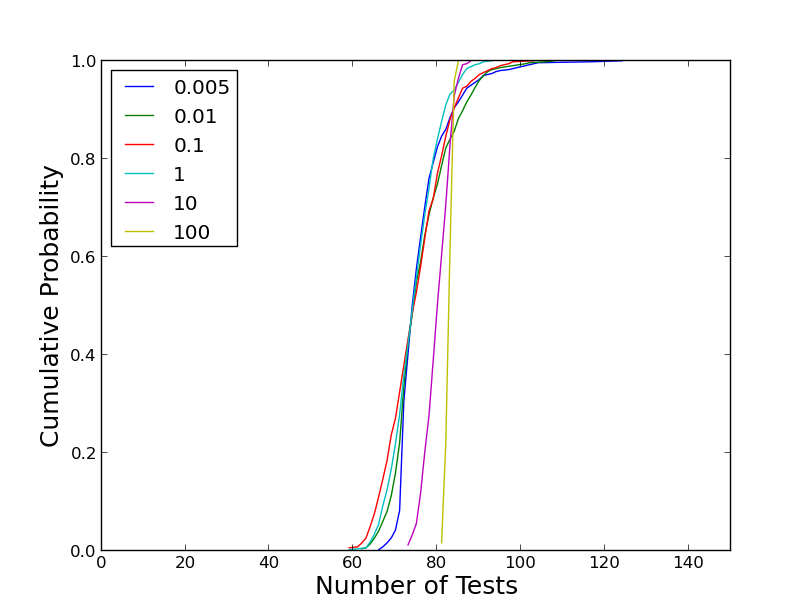
\includegraphics[width=0.7\textwidth]{manyalphalabels.png}
\caption{Cumulative distribution curves with Huffman searching}
\end{figure}

\begin{figure}[h]
\centering
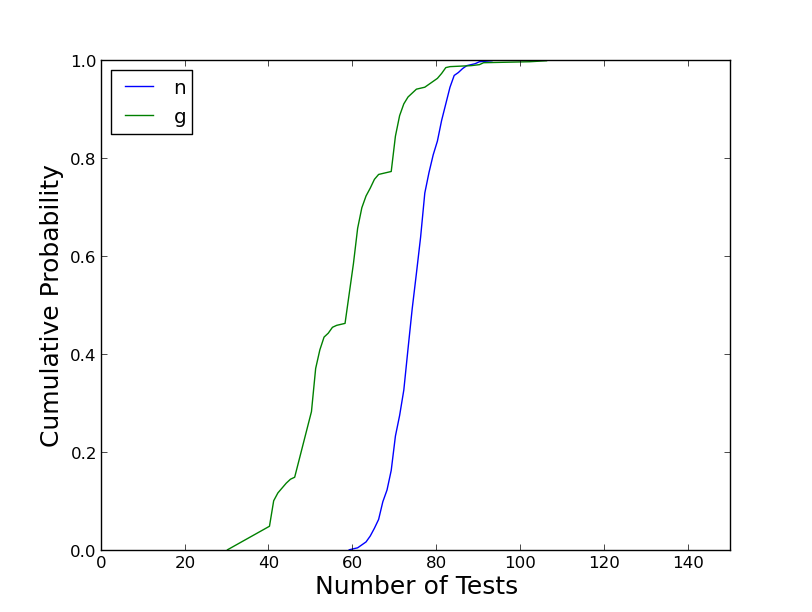
\includegraphics[width=0.7\textwidth]{greedyvnormal.png}
\caption{Cumulative distribution curves for greedy and normal pilot tests}
\end{figure}

\begin{figure}[h]
\centering
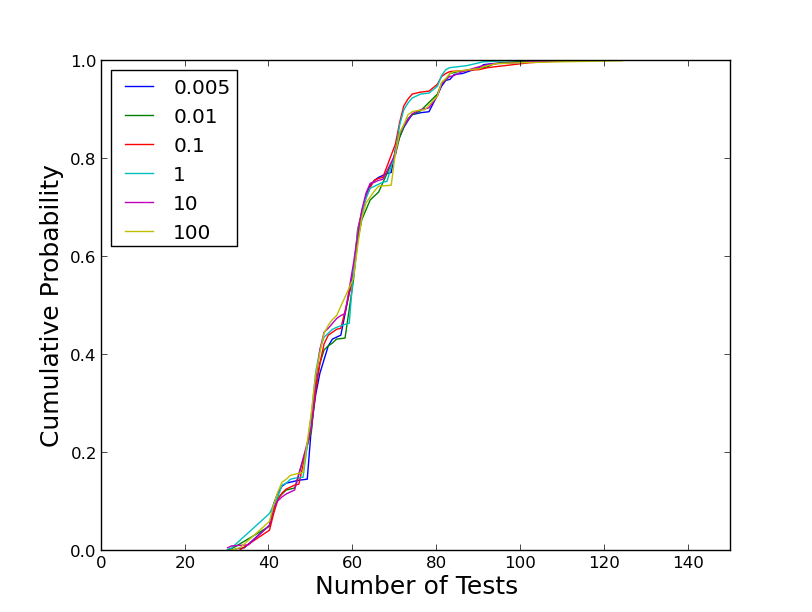
\includegraphics[width=0.7\textwidth]{manyalphagreedychoice.png}
\caption{Greedy pilot tests with varying alpha}
\end{figure}
\end{document}

\bibliographystyle{plain}
\bibliography{/users/tk12098/Documents/writing/quart-report.bib}
\end{document}